%\documentclass[twocolumn]{article}
%\usepackage[top=1.2cm, bottom=2cm, right=1cm, left=1cm]{geometry}
%\setlength{\columnsep}{20pt}
\documentclass{article}

\usepackage{hyperref,xcolor}
%\usepackage{algpseudocode}
\usepackage[lined,boxed]{algorithm2e}
\usepackage[english]{babel}
\usepackage{graphicx}
\usepackage{amsmath,amssymb}
\usepackage[utf8x]{inputenc}
\usepackage{graphicx}
\usepackage{subfigure}
\usepackage{dsfont}
\usepackage{url}
\usepackage{hyperref}
\usepackage{geometry}
\usepackage{mathrsfs}
%\usepackage[]{mcode}
\usepackage{color}
\usepackage{tikz}
\usetikzlibrary{arrows, decorations.markings}
\usetikzlibrary{shapes.geometric}
\usetikzlibrary{positioning}
\usetikzlibrary{fit}
\usepackage{sidecap}
\usepackage{bbold}
\usepackage{caption}
\usepackage{eurosym}
\usepackage{lipsum}

%\setlength\textwidth{\dimexpr 14cm + 1cm\relax}
%\setlength\columnsep{\dimexpr 1cm\relax}

\definecolor{wine-stain}{rgb}{0,0.4,0.2}
\hypersetup{
  colorlinks,
  linkcolor=wine-stain
}

\definecolor{magenta}{rgb}{1,0,1}
\definecolor{canard}{rgb}{0,1,1}
\definecolor{marron}{rgb}{0.9,0.4,0.1}
\definecolor{marron_noir}{rgb}{0.4,0.1,0}

\DeclareMathOperator*{\argmin}{\arg\!\min}
\DeclareMathOperator*{\argmax}{\arg\!\max}


\geometry{top=3cm , bottom=2.5cm}
\geometry{left=3cm , right=2.5cm}
%\geometry{left=1.5cm , right=1cm}

\title{\textbf{\textsc{Report: Milestone 2}}\vspace{4mm}}
\author{\textbf{Hou Yumeng, Alexis Jacq (Team $\mathbb{M}$)}\vspace{4mm}}

\begin{document}
%\lipsum
\maketitle

\section{Data Description}
Similar to the previous dataset we had for milestone 1, we have one dataset about 5478 users’ events (behaviours) on MOOC within 4 weeks, and another data file containing their final grades. Our mission is to predict the students’ grades based on their behaviours.

\section{Feature extraction}

\subsection{Week Labelling and Aggregation}
Firstly, we labelled the events in different weeks, and take them as individual features. \\
Then, we applied aggregation for users’ events during the four weeks. We aggregate and harvest the number of Unique behaviors \& Total behaviors (based on EventID). 
\subsection{Exploring New Features}
\subsubsection{Normal Feature Selection}
We added new features of Unique \textit{Video.$*$} events (\textit{Load, Play, Seek, Pause, SpeedChange}), Unique \textit{Forum.Load}, Unique \textit{Problem.Check} and Total \textit{Problem.Check}, most of which have around or above 0.5 correlation coef with final grades.
\subsubsection{Exploration Combinations As New Features}
We found the the proportion of submission times: $\textit{Unique.Problem.Check} / (\textit{Total.Problem.Check} + 1)$\\ helps in the prediction, so we took it as a new feature.\\
The interactions between solving problems and watching videos or launching in forum, as shown below, are correlated with the grades. So we added these features. \\
$\textit{Problem.Check} *\textit{Video.Load}$  \\ $\textit{Problem.Check} / (1+\textit{Forum.Thread.Launch})$
\subsubsection{Dealing With Submission TimeStamp}
We separated the submissions of each student into 4 weeks. In each week, we calculate the average submission TimeStamp / Maximum TimeStamp (of the week). If one didn't submit for a quiz, we take the maximum TimeStamp.
After getting the average submission time in each week, we calculated an average of these four results and take all these 5 values as new features.
We defined a new feature which normalizes the timestamps with the number of submissions given by \textit{Unique.Problem.Check}, in order to focus on the speed of students to submit:\\
$\textit{Speed} = \textit{SubmissionTime}/(1+\textit{Unique.Problem.Check})$\\

\section{Normalization}
Data normalization could be done by PCA and down-sampling/up-sampling, which were quite helpful to improve the results in training with sophisticated models. But it proved no help in simple linear regression. Hence we discarded it in our solution. 

\section{Model and Parameters}
We tried a variety of models including NNET, GBM, LM, RF, SVM, LDA, etc. We tuned the parameters accordingly based on the features of each model. We compared the performance mainly based on RMSE method but also the points got on KAGGLE. Though we kept improving slightly with better parameters (adjusting tuneGrid function). We finally surprisingly found that the simplest linear regression model with good features outperformed other "advanced" models greatly. We used stepwise approach by AIC to remove useless variables and to train our linear model.  

\section{Outliers Removal} 
We removed outliers after a first linear regression, which performed better than removal in the beginning. We used the distance between predicted grades derived from the first iteration and real grades, and removed the 0.1\% 
farthest points from the training set and re-applied a second linear regression.

\section{Visualization: Performance (RMSE) Comparison}
	\begin{figure}[!htb]
		\centering
 		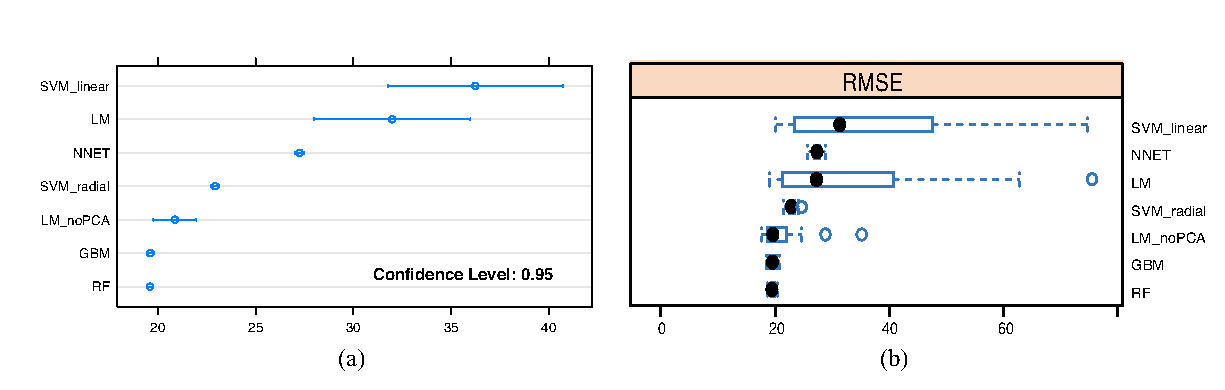
\includegraphics[width=1\linewidth]{Rplot2.eps}
 		\caption{Dotplot(a) and Boxplot(b) for RMSE of different models. }
 		\label{fig:rplot2}
	\end{figure}

As shown in Figure\ref{fig:rplot2}, we compared the models we used in terms of RMSE. When roughly tuned, random forest and GBM outperform the others. Linear Regression without PCA is also efficient but not so stable as the two models above. PCA proves no help for simple linear regression. Complex models such as SVM and NNET don't work well in this case and they're hard to tune as well. 

\end{document}

